\section{Wellen}
%\begin{itemize}
%    \setlength\itemsep{1pt}
%    \item Ausbreitungsphänomen von E und H
%    \item Ausbreitungsgeschw. kleiner $c_0$
%    \item raumzeitlicher Vorgang $cos(\omega t- \beta z)$
%    \item Energie- ohne Materietransport
%    \item Poyntingvektor $\vec{S}=\vec{E}\times\vec{H}$ Einheit[S]$= \dfrac{W}{m^2}$\\
%          {\footnotesize Falls $\vec{E}\perp\vec{H}$ und $\vec{S}\perp\vec{E}$ und $\vec{S}\perp\vec{H}$}
%\end{itemize}

%
%$\alpha$ : Dämpfungskonstante [Np/m]
%
%$\beta$ : Phasenkonstante [rad/m]
%
%$v_p$ : Phasengeschwindigkeit [m/s]
%
%$v_g$ : Gruppengeschwindigkeit [m/s]
%
%$\lambda$ : Wellen [m]

\subsection{Wellengleichungen allgemein}
\subsubsection{Zeitbereich}
auch d'Alembertsche Gleichungen genannt:
\begin{align*}
	\Delta \vec{E} -\kappa \mu \cdot \frac{\partial \vec{E}}{\partial t}-\varepsilon \mu \cdot \frac{\partial^2 \vec{E}}{\partial^2 t}& = \operatorname{grad} \frac{\rho}{\varepsilon} \\
	\Delta \vec{H} -\kappa \mu \cdot \frac{\partial \vec{H}}{\partial t}-\varepsilon \mu \cdot \frac{\partial^2 \vec{H}}{\partial^2 t}& = 0
\end{align*}
\subsubsection{Frequenzbereich}
auch Helmholtz-Gleichungen genannt:\\
mit harmonischer Zeitabhängigkeit: $ \frac{\partial }{\partial t} \rightarrow \mathrm{j}\omega $
\begin{align*}
	\Delta \underline{\vec{E}}-\left(\kappa \mu \cdot \mathrm{j} \omega-\varepsilon \mu \cdot \omega^{2}\right) \cdot \underline{\vec{E}} & = \operatorname{grad} \frac{\rho}{\varepsilon} \\
	\Delta \underline{\vec{H}}-\left(\kappa \mu \cdot \mathrm{j} \omega-\varepsilon \mu \cdot \omega^{2}\right) \cdot \underline{\vec{H}} & = 0
\end{align*}

\subsubsection{Vereinfachung der Gleichungen}
Bei quellfreiem, idealem Dielektrikum: $ \rho = \kappa = \vec{J} = 0$
\begin{align*}
	\Delta \vec{E}-\varepsilon \mu \frac{\partial^{2} \vec{E}}{\partial t^{2}} & =0 & 
	\Delta \vec{H}-\varepsilon \mu \frac{\partial^{2} \vec{H}}{\partial t^{2}} & =0 &\\
	\Delta \underline{\vec{E}}+\varepsilon \mu \omega^{2} \cdot \underline{\vec{E}} & =0 &
	\Delta \underline{\vec{H}}+\varepsilon \mu \omega^{2} \cdot \underline{\vec{H}} & =0 &
\end{align*}
Im elektrisch guten Leiter $\rho = 0,\, \kappa \gg \omega \epsilon$
\begin{align*}
	\Delta \vec{E}-\kappa \mu \frac{\partial^{2} \vec{E}}{\partial t^{2}} & =0 & 
	\Delta \vec{H}-\kappa \mu \frac{\partial^{2} \vec{H}}{\partial t^{2}} & =0 &\\
	\Delta \underline{\vec{E}}-\kappa \mu \omega^{2} \cdot \underline{\vec{E}} & =0 &
	\Delta \underline{\vec{H}}-\kappa \mu \omega^{2} \cdot \underline{\vec{H}} & =0 &
\end{align*}
%\textbf{Zeitabhängigkeit harmonisch:}
%\begin{align*}
%	\Delta \vec{H}   & = (j \omega \mu \sigma - \omega^2 \varepsilon \mu ) \vec{H}                                  \\
%	\Delta \vec{E} i & = (j \omega \mu \sigma - \omega^2 \varepsilon \mu ) \vec{E} + grad \frac{ \rho}{\varepsilon}
%\end{align*}

%\textbf{keine Raumladung $ \rho = 0$}
%\begin{align*}
%	\Delta \vec{E} & = (j \omega \mu \sigma - \omega^2 \varepsilon \mu ) \vec{E}
%\end{align*}

\subsection{Ebene Wellen}
Vereinfachung: harmonische Zeitabhängigkeit, keine Raumladungen $ \rho = 0 $, keine Feldstärkekomponenten in Ausbreitungsrichtung $ \frac{\partial^2 }{\partial^2 x} = \frac{\partial^2 }{\partial^2 y} = 0 $
\begin{align*}
	\Delta \vec{E} & = \frac{ \partial \vec{E}}{ \partial z^2} = j \omega \mu ( \kappa + j \omega \varepsilon) \vec{E} \\
	\Delta \vec{H} & = \frac{ \partial \vec{E}}{ \partial z^2} = j \omega \mu ( \kappa + j \omega \varepsilon) \vec{H}
\end{align*}

\textbf{TEM}-Welle: $\vec{E}$ und $ \vec{H} $ besitzen nur transversale (= \textit{senkrecht zur Ausbreitungsrichtung} stehende) Komponenten.
%%%%%%%%%%%%%%%%%

\subsubsection{Gleichung Ebene Welle}
Tatsächlicher Zeitverlauf (\textbf{Realteil} von $\underline{\vec{E}}(z,t)$)
\begin{empheq}[]{align*}
	\boxed{\vec{E}(z,t)
		= \underbrace{E_0}_{\mathclap{\text{Amplitude}}}
		\cdot \overbrace{e^{-\alpha z}}^{\mathclap{\text{Dämpfung}}}
		\cdot \underbrace{cos(\omega t \overbrace{-}^{\mathclap{\text{positive z-Richtung}}} \beta z)}_\text{Zeit- und Raumabhängigkeit}
		\cdot\vec{e}_z}
\end{empheq}

\subsubsection{komplexer Amplitudendrehzeiger}
Achtung: \textbf{mit} $ e^{jwt} $ ! , wenn \textbf{ohne}: komplexer Amplituden\textit{vektor}.
\begin{empheq}[]{align*}
	\boxed{\underline{\vec{E}}(z,t)
		= E_0\cdot e^{-\alpha z}\cdot e^{j(\omega t-\beta z)}\cdot\vec{e}_z
		= E_0\cdot e^{-\underline{\gamma}z}\cdot e^{j\omega t}\cdot\vec{e}_z
	}
\end{empheq}
\subsubsection{Fortpflanzungskonstante}
Dämpfungskonstante $ \alpha $: $\frac{\mathtt{Np}}{m}$ \qquad \quad
Phasenkonstante $ \beta $: $ \frac{\mathtt{rad}}{m} $
\[\underline{\gamma}=\alpha+j\beta \quad \left[ \frac{1}{m} \right] \]
%\newcolumn
\subsection{Kenngrößen}
\subsubsection{Wellenzahl}
Im Vakuum: $k_{0}=\dfrac{\omega}{c_{0}}$
\begin{align*}
	\beta \, \widehat{=} \, k & = \frac{\omega}{v_p} = \frac{2\pi}{\lambda} = \frac{2 \pi f}{v_p} = |\vec{k}| \quad \left[ \frac{\texttt{rad}}{\texttt{m}}\right]                                                                     \\
	& = \frac{\omega \cdot n}{c_{0}} = n \cdot k_{0}=\sqrt{\mu_{r} \cdot \varepsilon_{r}} \cdot k_{0} = k_{r} \cdot k_{0}
\end{align*}

\subsubsection{Wellenlänge}
Periodenlänge entlang der Ausbreitungsrichtung.\\
Freiraumwellenlänge: im materiefreien Raum $ \lambda_0 $
\begin{align*}
	\lambda_0 & = \dfrac{c_0}{f} = \dfrac{2\pi}{k_0} \quad [\texttt{m}]\\
	\lambda   & = \dfrac{\lambda_0}{\sqrt{\mu_r \cdot \varepsilon_r}} = \dfrac{2 \pi}{k} = \dfrac{v_p}{f} = \dfrac{\lambda_0}{n} = \dfrac{2 \pi}{n \cdot k_0}
\end{align*}

\subsubsection{Phasengeschwindigkeit}
\[
v_p = \dfrac{d z}{d t} = \dfrac{\omega}{k} = \frac{1}{\sqrt{ \mu_r \mu_0 \varepsilon_r \varepsilon_0} } = \frac{c_0}{\sqrt{\mu_r \varepsilon_r}} \qquad v_{p,\texttt{Medium} \leq c_0}
\]

\subsubsection{Brechzahl/Brechungsindex}
\[ 
n = \frac{c_0}{v_p} = \sqrt{\mu_r \varepsilon_r} \approx \sqrt{\varepsilon_r} \geq 1
 \]
\subsubsection{Gruppengeschwindigkeit}
\[
v_g = \dfrac{d \omega}{d k} \widehat{=} \dfrac{\textnormal{Wegstück der Wellengruppe}}{\textnormal{Laufzeit der Wellengruppe}}
\]
%\begin{align*}
%	E_1(z,t)   & = E\cos((\omega_0-\Delta\omega)t-(\beta_0-\Delta\beta)z)                                                                                                                                     \\
%	E_2(z,t)   & = E\cos((\omega_0+\Delta\omega)t-(\beta_0+\Delta\beta)z)                                                                                                                                                                                                                                                                                                                             \\
%	\Rightarrow E(z,t)     & = 2E\cdot\underbrace{\cos(\omega_0t-\beta_0z)}_{\mathclap{\text{Grundfrequenz $\omega$}}}\cdot\underbrace{\cos(\Delta\omega t-\Delta\beta z)}_{\mathclap{\text{Einhüllende $\Delta\omega$}}} \\
%	v_p        & = \frac{\omega_0}{\beta_0}          \qquad                                                                                                                                                         
%	v_g        = \frac{\Delta\omega}{\Delta\beta}
%\end{align*}

\subsubsection{Feldwellenwiderstand}
$ Z_{F0} $: im \textbf{materiefreien} Raum/Vakuum!\\
Falls keine Verluste (ideal) $ \rightarrow Z_F $ reell!
\begin{align*}
	\underline{Z}_F &= \frac{\underline{E}_{\texttt{transversal}}}{\underline{H}_{\texttt{transversal}}} = \frac{\underline{E}_h}{\underline{H}_h} = -\frac{\underline{E}_r}{\underline{H}_r} = \frac{\omega \mu}{\underline{k}} = \sqrt{\frac{j\omega\mu}{\kappa+j \omega \varepsilon}}\\
	Z_{F0} &= \sqrt{\frac{\mu_0}{\varepsilon_0}} = 120\pi \Omega \qquad  Z_F = Z_{F0} \cdot \sqrt{\frac{\mu_r}{\varepsilon_r}} &
\end{align*}
\subsubsection{Poynting-Vektor}
gibt Leistungsfluss einer EM-Welle und Richtung der Energieströmung an.\\
\begin{tabular}{|l|l|}
	\hline
	Zeitbereich & Frequenzbereich\\
	\hline
	$\vec{S} = \vec{E} \times \vec{H}$ & $\vec{\underline{S}} = \frac{1}{2} (\underline{\vec{E}} \times \underline{\vec{H}}^*)$ \\
	$\vec{S}_{av} = \overline{\vec{S}(t)} = \frac{1}{T} \int_{0}^{T} \vec{S}(t) \,dt $ & $\vec{S}_{av} = \frac{1}{2} \Re{\underline{\vec{E}} \times \underline{\vec{H}}^*}$\\
	\hline
	\multicolumn{2}{|c|}{Leistungsflussdichte, Intensität $\quad S_{av} = |\vec{S}_{av}|$}\\
	\hline
\end{tabular}
\begin{align*}
%	\vec{S}             & =  \vec{E}\times\vec{H} \qquad \si{\left[\frac{W}{m^2}\right]} \\
%	\vec{S}_{\text{av}} & =  \frac{1}{2} \cdot Re\{\vec{E}\times\vec{H}^*\}              \\
	S_{av}              & =  \frac{1}{2} \cdot E \cdot H 
	=  \frac{1}{2} \cdot \dfrac{E^2}{Z_{F0}}            
	=  \frac{1}{2} \cdot H^2 \cdot Z_{F0} 
	=  \frac{P}{A_\texttt{Fläche}}\\
	P &= \iint\vec{S}_{\text{av}}\, d\vec{a}                
	= Re\left\{\underline{U}\cdot\underline{I}^*\right\}\\
	P_1 & = P_0 \cdot e^{-2\alpha z} \qquad P_{\texttt{Leitung}} = \dfrac{1}{2} \dfrac{\hat{U}^2}{\cdot \Re{Z_L}}
%	w_{e} & = \frac{1}{2}\cdot\mu\cdot H^2              
%	&w_{e} & = \frac{1}{2}\cdot\varepsilon\cdot E^2&
\end{align*}
\newcolumn
\subsection{Ausbreitung im Medium}
$ \kappa, \sigma $ = Leitfähigkeit
\subsubsection{Allgemein (mit Verlusten)}
\begin{align*}
    \lambda                 & = \dfrac{2\pi}{\beta} \qquad E_2 = E_1 e^{-\alpha z}         \qquad                                                                            
    v_p                      = \lambda\cdot f = \dfrac{\omega}{\beta}                                                                                                    \\
    \alpha                  & = \omega \cdot \sqrt{\dfrac{\mu \varepsilon}{2}\cdot \left(\sqrt{1+\dfrac{\sigma^2}{\omega^2\cdot\varepsilon^2}}{\color{red}{-}}1\right)}   \\
    \beta                   & = \omega \cdot \sqrt{\dfrac{\mu \varepsilon}{2}\cdot \left(\sqrt{1+\dfrac{\sigma^2}{\omega^2\cdot\varepsilon^2}}{\color{green}{+}}1\right)} \\
    \Aboxed{\underline{Z}_F & = \dfrac{\underline{E}}{\underline{H}} = \sqrt{\dfrac{j\omega\mu}{\sigma+j\omega\varepsilon}}}
\end{align*}

\subsubsection{Im leeren Raum (Vakuum)}
materiefreier Raum: $ \mu_r = \varepsilon_r = 1 $
\begin{align*}
    \alpha                     & = 0 &
    \beta                      & = \dfrac{\omega}{c_0} \qquad 
    \lambda_0                   = \dfrac{c_0}{f} \\
    v_p                        & = c_0 &
Z_{F0} & = \sqrt{\dfrac{\mu_0}{\varepsilon_0}} = 120 \pi\Omega\approx377\Omega &
\end{align*}
\subsubsection{Im verlustlosen Dielektrikum}
verlustlos: $\kappa =0$, maximale Wirkleistung\\
$Z_F$ rein reell $\rightarrow$ ebene Welle
\begin{align*}
    \alpha                  & = 0 &
    \beta                   & = \dfrac{\omega}{c_0}\sqrt{\mu_r\varepsilon_r}=\omega\sqrt{\mu\varepsilon}=\dfrac{2\pi}{\lambda} \\
    \lambda                 & = \dfrac{c_0}{f}\dfrac{1}{\sqrt{\mu_r\varepsilon_r}} &
    v_p                     & = \dfrac{c_0}{\sqrt{\mu_r\varepsilon_r}}         \qquad
    \boxed{Z_F = \sqrt{\dfrac{\mu}{\varepsilon}}=Z_{F0}\sqrt{\frac{\mu_r}{\varepsilon_r}}}
\end{align*}

\subsubsection{Im Dielektrika mit geringem Verlust}
geringer Verlust: $0 < \kappa \ll\omega\varepsilon$
\begin{align*}
    \alpha                  & \approx\dfrac{\sigma}{2}\cdot\sqrt{\dfrac{\mu}{\varepsilon}} = \frac{\sigma}{2}\cdot Z_{F0}\sqrt{\frac{\mu_r}{\varepsilon_r}}  \quad 
    \beta \approx\omega\sqrt{\mu\varepsilon}\left(1+\dfrac{1}{8}\cdot\dfrac{\sigma^2}{\omega^2\varepsilon^2}\right)                                                  \\
    \lambda                 & = \dfrac{c_0}{f}\cdot\dfrac{1}{\sqrt{\mu_r\varepsilon_r}}\cdot\frac{1}{1+\frac{1}{8}\left(\frac{\sigma}{\omega\varepsilon}\right)^2}                       \\
    v_p                     & = \dfrac{c_0}{\sqrt{\mu_r\varepsilon_r}}\cdot\frac{1}{1+\frac{1}{8}\left(\frac{\sigma}{\omega\varepsilon}\right)^2}                                        \\
    \Aboxed{\underline{Z}_F & = \sqrt{\dfrac{\mu}{\varepsilon}}\left(1-\frac{j\sigma}{\omega\varepsilon}\right)^{-^1/2} \approx Z_{F0}\left(1+\frac{j\sigma}{2\omega\varepsilon}\right)}
\end{align*}

\subsubsection{Im guten Leiter}
geringer Verlust: $\sigma \gg\omega\varepsilon$
\begin{align*}
    \alpha                  & \approx \beta \approx\sqrt{\frac{\omega\mu\sigma}{2}}=\dfrac{1}{\delta}\sim\sqrt{f} \qquad
    \lambda                 = 2\pi \sqrt{\dfrac{2}{\omega\mu\sigma}}=2\pi\delta                                 \\
    v_p                     & = \frac{2\pi}{\beta} = \omega\delta        \qquad                                        
    \boxed{\underline{Z}_F = \sqrt{\dfrac{j\omega\mu}{\sigma}} \approx \dfrac{1+j}{\sigma\cdot\delta} = \sqrt{\frac{\omega \mu}{\kappa}}e^{\mathrm{j}\frac{\pi}{4}}   }
\end{align*}
%\newpage
\subsection{Ebene Wellen an Grenzflächen}
\subsubsection{Zwischen Dielektrika mit geringem Verlust}

\begin{center}
    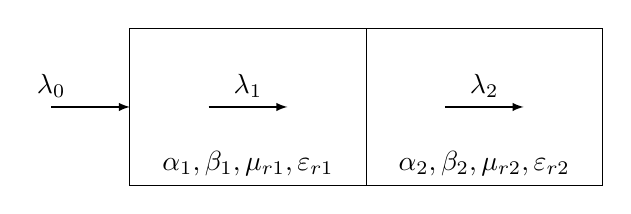
\begin{tikzpicture}
        %arrows
        \draw[-latex](0,1)--(1,1) node at (0,1)[above]{$\lambda_0$};
        \draw[-latex](2,1)--(3,1) node [midway, above]{$\lambda_1$};
        \draw[-latex](5,1)--(6,1) node [midway, above]{$\lambda_2$};

        %frame
        \draw[-](1,0)--(4,0) node [midway, above]{$\alpha_1, \beta_1, \mu_{r1}, \varepsilon_{r1}$};
        \draw[-](4,0)--(7,0) node [midway, above]{$\alpha_2, \beta_2, \mu_{r2}, \varepsilon_{r2}$};
        \draw[-](1,2)--(7,2);
        \draw[-](1,0)--(1,2);
        \draw[-](4,0)--(4,2);
        \draw[-](7,0)--(7,2);
    \end{tikzpicture}
\end{center}
% \includegraphics[width=\columnwidth]{Figures/UebergangzweiDielektrika.png}
\begin{align*}
    \quad \qquad \lambda_1 & = \dfrac{\lambda_0}{\sqrt{\mu_{r1}\varepsilon_{r1}}}          & \lambda_2 & = \dfrac{\lambda_0}{\sqrt{\mu_{r2}\varepsilon_{r2}}}                                     \\
    \quad \qquad           &                                                               &           & = \dfrac{\lambda_1\cdot\sqrt{\mu_{r1}\varepsilon_{r1}}}{\sqrt{\mu_{r2}\varepsilon_{r2}}} \\
    \quad \qquad \beta_1   & = \dfrac{2\pi}{\lambda_0}\cdot\sqrt{\mu_{r1}\varepsilon_{r1}} & \beta_2   & = \dfrac{2\pi}{\lambda_0}\cdot\sqrt{\mu_{r2}\varepsilon_{r2}}                            \\
    \quad \qquad Z_{F1}    & = \dfrac{Z_{F0}}{\sqrt{\mu_{r1}\varepsilon_{r1}}}             & Z_{F2}    & = \dfrac{Z_{F0}}{\sqrt{\mu_{r2}\varepsilon_{r2}}}
\end{align*}

%\subsection{Poyntingvektor}
%gibt Leistungsfluss einer EM-Welle und Richtung der Energieströmung an.\\
%
%\begin{tabular}{|l|l|}
%\hline
%Zeitbereich & Frequenzbereich\\
%\hline
%$\vec{S} = \vec{E} \times \vec{H}$ & $\vec{\underline{S}} = \frac{1}{2} (\underline{\vec{E}} \times \underline{\vec{H}}^*)$ \\
%$\vec{S}_{av} = \overline{\vec{S}(t)} = \frac{1}{T} \int_{0}^{T} \vec{S}(t) \,dt $ & $\vec{S}_{av} = \frac{1}{2} \Re{\underline{\vec{E}} \times \underline{\vec{H}}^*}$\\
%\hline
%\multicolumn{2}{|c|}{Leistungsflussdichte $\quad S_{av} = |\vec{S}_{av}|$}\\
%\hline
%\end{tabular}

%\begin{align*}
%    \vec{S}             & =  \vec{E}\times\vec{H} \qquad \si{\left[\frac{W}{m^2}\right]} \\
%    \vec{S}_{\text{av}} & =  \frac{1}{2} \cdot Re\{\vec{E}\times\vec{H}^*\}              \\
%    S_{AV}              & =  \frac{1}{2} \cdot E \cdot H =                               \\
%                        & =  \frac{1}{2} \cdot \dfrac{E^2}{Z_{F0}} =                     \\
%                        & =  \frac{1}{2} \cdot H^2 \cdot Z_{F0}                          \\
%                        & =  \dfrac{P}{A_\texttt{Fläche}}                                \\
%\end{align*}

%\subsubsection{Leistung}
%
%\begin{align*}
%    P     & = \iint\vec{S}_{\text{av}}d\vec{a}                   \\
%          & = Re\left\{\underline{U}\cdot\underline{I}^*\right\} \\
%    w_{e} & = 1/_2\cdot\mu\cdot H^2                              \\
%    w_{e} & = 1/_2\cdot\varepsilon\cdot E^2
%\end{align*}

%\subsubsection{Leistung vom Kabel transportiert}
%
%\begin{align*}
%    P & = \dfrac{\hat{U}^2}{2\cdot Z_L}
%\end{align*}

%\subsection{dÀlembertsche Gleichung (allg.)}
%\begin{align*}
%    \Delta \vec{E}-\kappa \mu \frac{\partial \vec{E}}{\partial t}-\varepsilon \mu \frac{\partial^{2} \vec{E}}{\partial t^{2}} & = \operatorname{grad} \frac{\rho}{\varepsilon} \\
%    \Delta \vec{H}-\kappa \mu \frac{\partial \vec{H}}{\partial t}-\varepsilon \mu \frac{\partial^{2} \vec{H}}{\partial t^{2}} & = 0
%\end{align*}
%
%Isolator, ideales Dielektrikum, Nichtleiter $\kappa = 0$
%\begin{align*}
%    \Delta \vec{E} & =\varepsilon \mu \frac{\partial^{2} \vec{E}}{\partial t^{2}}+\operatorname{grad} \frac{\rho}{\varepsilon} \\
%    \Delta \vec{H} & =\varepsilon \mu \frac{\partial^{2} \vec{H}}{\partial t^{2}}
%\end{align*}

%sehr gute Leiter
%\begin{align*}
%    \Delta \vec{E} & =\kappa \mu \frac{\partial \vec{E}}{\partial t}+\operatorname{grad} \frac{\rho}{\varepsilon} \\
%    \Delta \vec{H} & =\kappa \mu \frac{\partial \vec{H}}{\partial t}
%\end{align*}

%\subsection{Polarisation}
%\begin{tabularx}{0.45\textwidth}{>{\hsize=.27\hsize}X|>{\hsize=.5\hsize}X|>{\hsize=.23\hsize}X}
%    Lineare      & wenn der Endpunkt des E–Vektors eine Linie beschreibt & $H$ oder $E$ \\
%    \hline
%    Elliptische  & Endpunkt des E-Vektors eine Ellipse beschreibt        & $E\neq H$    \\
%    \hline
%    Kreisförmige & der Endpunkt des E-Vektors einen Kreis beschreibt     & $E = H$      \\
%\end{tabularx}



%\subsubsection{Totalrefexion/Grenzwinkel}
%Grenzwinkel $ \theta_g $ gibt an, bis zu welchem Winkel eine Welle von höherem in kleineres Dielektrikum $ \varepsilon_1 > \varepsilon_2 $ eindringen kann.
%\begin{align*}
%    \sin\theta_g & = \frac{n_2}{n_1} = \sqrt{\frac{\mu_{r2}\varepsilon_{r2}}{\mu_{r1}\varepsilon_{r1}}}
%\end{align*}
%\begin{align*}
%    \alpha_g & = \sin^{-1} \left( \sqrt{ \dfrac{\mu_{r1} \varepsilon_{r1}}{\mu_{r2} \varepsilon_{r2}}} \right)
%\end{align*}
%\subsubsection[Brewster-/Polarisationswinkel]{Brewster-/Polarisationswinkel}
%Bei Brewster-Winkel $ \theta_b $ wird Reflexionsfaktor $r=0$.
%\begin{itemize}
%%    \item Snelliusche Brechungsgesetz
%          %\item Grenzwinkel $\alpha_g$
%          % \item[--] Brewsterwinkel $\alpha_B$ (Welle transmittiert reflexionsfrei)
%          %       \begin{itemize}
%          %           \item[\textbullet] Parallele Polarisation (Nur wenn $\mu_{r1} = \mu_{r2}$)
%          %           \item[\textbullet] Senkrechte Polarisation (Nur wenn $\varepsilon_{r1} = \varepsilon_{r2}$)
%          %       \end{itemize}
%    \item Paralleler Reflexionskoeffizient:
%          \begin{align*}
%              \Aboxed{\mu_{r1}=\mu_{r2}}                                                                                                    \\
%              \sin\theta_b & = \sqrt{\frac{\varepsilon_2(\mu_2\varepsilon_1 - \mu_1\varepsilon_2)}{\mu_1(\varepsilon_1^2-\varepsilon_2^2)}} \\
%              \tan\theta_b & = \sqrt{\frac{\varepsilon_2}{\varepsilon_1}} = \frac{n_2}{n_1}
%          \end{align*}
%
%    \item Senkrechter Reflexionskoeffizient:
%          \begin{align*}
%              \Aboxed{\varepsilon_{r1}=\varepsilon_{r2}}                                                                    \\
%              \sin\theta_b & = \sqrt{\frac{\mu_2(\mu_2\varepsilon_1 - \mu_1\varepsilon_2)}{\varepsilon_1(\mu_2^2-\mu_1^2)}} \\
%              \tan\theta_b & = \sqrt{\frac{\mu_2}{\mu_1+\mu_2}}
%          \end{align*}
%\end{itemize}
\subsubsection{Brechungsgesetz allgemein}
\begin{align*}
    \dfrac{\sin \vartheta_{2}}{\sin \vartheta_{1}} = \dfrac{k_{h}}{k_{g}} & = \sqrt{\dfrac{\mu_{r 1} \varepsilon_{r 1}}{\mu_{r 2} \varepsilon_{r 2}}} = \dfrac{n_{1}}{n_{2}} = \dfrac{v_{p, 2}}{v_{p, 1}} = \dfrac{\lambda_{2}}{\lambda_{1}} \\
    % \alpha_{Bp}                                                           & = \tan^{-1} \left( \sqrt{ \dfrac{\varepsilon_{r1}}{\varepsilon_{r2}}} \right)                                                                                        \\
    % \alpha_{Bs}                                                           & = \tan^{-1} \left( \sqrt{ \dfrac{\mu_{r1}}{\mu_{r2}}} \right)
\end{align*}

\subsubsection{Leistungsbilianz an Grenzflächen}
Index n: Normalkomponente. Wichtig: Beträge beachten!
\begin{align*}
	S_{tn} &= S_{hn} - S_{rn}\\ 
	S_{t0} &= S_{h0}\cdot \frac{\cos\vartheta_{1}}{\cos\vartheta_{2}}(1-r^2)
\end{align*}

\subsection{Polarisation einer Welle}
Die Polarisation (Ausrichtung) bezieht sich \textbf{immer} auf das $\vec{E}$-Feld.
\begin{itemize}
	\item \textbf{Lineare} Polarisation\\
	Endpunkt des $\vec{E}$-Vektors beschreibt bei fortschreitender Welle eine Gerade (Linie).
		\begin{itemize}
			\item horizontale Polarisation: E-Feld parallel zum Erdboden.
			\item vertikale Polarisation E-Feld senkrecht zum Erdboden.
		\end{itemize}
	\item \textbf{Elliptische} Polarisation\\
	Endpunkt des $\vec{E}$-Vektors beschreibt bei fortschreitender Welle eine Ellipse.
		\begin{itemize}
			\item Zirkulare Polarisation: $|\vec{E}_x| = |\vec{E}_y|$ bei $ \vec{E}_x \perp \vec{E}_y $ ($ \ang{90}$ Phasenverschiebung)
		\end{itemize}
\end{itemize}



%\subsection{Polarisation}
\
\subsection[Senkrechter Einfall]{Senkrechter Einfall}
Gilt bei Einfallswinkel $ \theta_h = 0 $.
\begin{center}
    \tikzset{cross/.style={cross out, draw=black, minimum size=2*(#1-\pgflinewidth), inner sep=0pt, outer sep=0pt},
        %     %default radius will be 1pt. 
        cross/.default={3.5pt}}
    \begin{tikzpicture}
        %Kreuz
        \draw[dotted] (-3,0) -- (3,0);
        \draw[-] (0,-2.5) -- (0,2.5)                        node[below left] {Medium 1} 
                                                            node[below right] {Medium 2}
                                                            node at (0,-2.5)[above left] {$\varepsilon_1, \mu_1, \sigma_1$}
                                                            node at (0,-2.5)[above right] {$\varepsilon_2, \mu_2, \sigma_2$};
        %Rücklaufende
        \draw[-latex] (-2,1.5) -- (-3,1.5)                  node[above] {$S_r$};
        \draw[-latex] (-2,1.5) -- (-2,2.5)                  node[above] {$E_r$};
        \draw[-] (-2,1.5) circle (0.15)                     node[below right] {$H_r$};
        \draw(-2,1.5) node [cross] {};
        \draw[dotted] (-3,1.5) -- (0,1.5);

        %Hinlaufende
        \draw[dotted] (-3,-1.5) -- (0,-1.5);
        \draw[-latex] (-2,-1.5) -- (-1,-1.5)                node[above left] {$S_h$};
        \draw[-latex] (-2,-1.5) -- (-2,-0.5)                node[above] {$E_h$};
        \draw[-] (-2,-1.5) circle (0.15)                    node[below right] {$H_h$};
        \draw[-,fill=black!100] (-2,-1.5) circle (0.05);

        %Transmitierte
        \draw[-latex] (2,0) -- (3,0)                        node[right] {$S_t$};
        \draw[-latex] (2,0) -- (2,1)                        node[below right] {$E_t$};
        \draw[-] (2,0) circle (0.15)                        node[below right] {$H_t$};
        \draw[-,fill=black!100] (2,0) circle (0.05);
        
%       Koordinatensystem!
		\draw[-latex] (2,-1.5) -- (2.5,-1.5)                node[right] {$z$};
      	\draw[-latex] (2,-1.5) -- (2,-1)                node[above] {$x$};
       	\draw[-] (2,-1.5) circle (0.15)                    node[below left] {$y$};
        \draw[-,fill=black!100] (2,-1.5) circle (0.05);
%		\draw[-latex] (-2,-1.5) -- (-2,-0.5)                node[above] {$E_h$};
%		\draw[-] (-2,-1.5) circle (0.15)                    node[below right] {$H_h$};
%		\draw[-,fill=black!100] (-2,-1.5) circle (0.05);

    \end{tikzpicture}
\end{center}
%$ E_{t1}=E_{t2} \qquad H_{t1} = H_{t2}$
\begin{equation*}
\setlength{\jot}{10pt}
\begin{aligned}[t]
%
	r_e &= \frac{Z_{F2}-Z_{F1}}{Z_{F2} + Z_{F1}}\\
	r_m &= \frac{Z_{F1}-Z_{F2}}{Z_{F2} + Z_{F1}}\\
	&=-r_e\\
\end{aligned}
\qquad \qquad
\begin{aligned}[t]
%	&0\leq t\leq2 &0\leq|r|\leq1&\\
	t_e  &= \frac{2 \cdot Z_{F2}}{Z_{F1} + Z_{F2}}\\ 
	t_m  &= \frac{2 \cdot Z_{F1}}{Z_{F1} + Z_{F2}} \\
	&= t_e \cdot \frac{Z_{F1}}{Z_{F2}}\\
\end{aligned}
\end{equation*}
%\begin{align*}
%    %\qquad = \frac{\sqrt{\varepsilon_{r2}}-\sqrt{\varepsilon_{r1}}}{\sqrt{\varepsilon_{r2}}+\sqrt{\varepsilon_{r1}}}
%\end{align*}
\vspace{-0.2cm}
%Elektrisches Feld:
\begin{equation*}
\setlength{\jot}{6pt}
\begin{aligned}[t]
	t_e & = 1+ r_e \\	
	E_{t1} & =E_{t2}\\
    E_t & = t_e \cdot E_h \\
	E_r & = r_e \cdot E_h \\
	E_t & = E_h + E_r \\        
	t_e\cdot E_{h} & = E_{h} + r_e\cdot  E_{h} \\
\end{aligned}
\qquad
\begin{aligned}[t]
	t_m & = 1+ r_m \\
	H_{t1} &= H_{t2}\\
	H_t & = t_e \cdot \tfrac{Z_{F1}}{Z_{F2}} \cdot H_h \\
	-H_r & = r_e \cdot H_h \\
	H_t & = H_h + H_r \\        
	t_m\cdot H_{h} & = H_{h} + r_m\cdot  H_{h} \\
\end{aligned}
\end{equation*}

%\begin{align*}
%\end{align*}
%
%Magnetisches Feld:

% \begin{align*}
%     r_m & = r = r_e                                                    \\
%     t_m & = \frac{2}{1+\sqrt{^{\varepsilon_{r1}}/_{\varepsilon_{r2}}}}
% \end{align*}
\begin{align*}
    %\vec{H_t}                   & = \vec{H_h}-\vec{H_r}                                \\
    H_t                         & = H_h + H_r                                          \\
    \frac{t\cdot E_{h}}{Z_{F2}} & = \frac{E_{h}}{Z_{F1}} - \frac{r\cdot E_{h}}{Z_{F1}} \\
    \frac{t}{Z_{F2}}            & = \frac{1}{Z_{F1}} - \frac{r}{Z_{F1}}
\end{align*}




\subsubsection[Senkrechter Einfall ideales/verlustl. Dielekt.]{Verlustloses Dielektikum allgemein}
gilt für $ \kappa =0 $, keine Dämpfung.
%\includegraphics[width=\columnwidth]{Figures/senkrechterEinfall.png}
%\vspace{-0.3cm}
\[ \text{rein reell: }Z_F=  \sqrt{\frac{\mu_0\mu_r}{\varepsilon_0\varepsilon_r}}  \qquad
\text{rein imaginär: }\gamma  = j \omega\sqrt{\mu\varepsilon} \]
%\vspace{-0.5cm}
\begin{align*}
    r & = r_e =\frac{Z_{F2} - Z_{F1}}{Z_{F1} + Z_{F2}} = \frac{\sqrt{\varepsilon_{r1}\mu_{r2}} - \sqrt{\varepsilon_{r2}\mu_{r1}} }{\sqrt{\varepsilon_{r1}\mu_{r2}}+{\sqrt{\varepsilon_{r2}\mu_{r1}}}} \\
    t & = t_e = \frac{2 Z_{F2}}{Z_{F1} + Z_{F2}} = \frac{2\sqrt{\varepsilon_{r1}\mu_{r2}}}{\sqrt{\varepsilon_{r1}\mu_{r2}}+\sqrt{\varepsilon_{r2}\mu_{r1}}}
\end{align*}
% \begin{tabularx}{\columnwidth}{>{\hsize=.35\hsize}X|>{\hsize=.32\hsize}X>{\hsize=.18\hsize}X>{\hsize=.18\hsize}X}
%     idealer Leiter    & $ Z_{F2} = 0 $                    & $ r = -1 $ & $t = 0$ \\
%     \hline
%     ideales Dielektr. & $\mu_{r1} = \varepsilon_{r1} = 1$ &            &         \\
% \end{tabularx}

\subsubsection{Medium 1 oder 2: Luft}
\begin{equation*}
	\setlength{\jot}{6pt}
	\begin{aligned}[t]
   		\Aboxed{ & \mu_{r1} = \varepsilon_{r1} = 1}                                                            \\
		r        & = \frac{\sqrt{\mu_{r2}}-\sqrt{\varepsilon_{r2}}}{{\sqrt{\mu_{r2}}+\sqrt{\varepsilon_{r2}}}} \\
		t        & = \frac{2\sqrt{\mu_{r2}}}{\sqrt{\mu_{r2}}+\sqrt{\varepsilon_{r2}}}
	\end{aligned}
	\qquad
	\begin{aligned}[t]
  		\Aboxed{ & \mu_{r2} = \varepsilon_{r2} = 1}                                                            \\
		r        & = \frac{\sqrt{\varepsilon_{r1}}-\sqrt{\mu_{r1}}}{{\sqrt{\varepsilon_{r1}}+\sqrt{\mu_{r1}}}} \\
		t        & = \frac{2\sqrt{\varepsilon_{r1}}}{\sqrt{\mu_{r1}}+\sqrt{\varepsilon_{r1}}}
	\end{aligned}
\end{equation*}

%\begin{align*}
%
%\end{align*}

%\subsubsection{Medium 2: Luft}
%\begin{align*}
%\end{align*}

\subsubsection{beide Medien: nicht magnetisch}
%\centering
Gilt für $\mu_{r1} = \mu_{r2} = 1$
\begin{align*}
    r        & = \frac{\sqrt{\varepsilon_{r1}}-\sqrt{\varepsilon_{r2}}}{{\sqrt{\varepsilon_{r1}}+\sqrt{\varepsilon_{r2}}}}&
    t        & = \frac{2\sqrt{\varepsilon_{r1}}}{\sqrt{\varepsilon_{r1}}+\sqrt{\varepsilon_{r2}}}&
\end{align*}

\subsubsection{Medium 2: idealer Leiter}
$\vec{E}=0$ im idealen Leiter $\rightarrow$ \textbf{Stehende} Welle!, vollständige Reflexion.
\begin{equation*}
	Z_{F2}       = 0 \qquad
	r            = -1 \qquad
	t            = 0 \qquad
	\vec{S}_{\text{av}} = 0
\end{equation*}
%\vspace{-0.8cm}
\begin{flalign*}
    &\underline{E}_{1x}          = -2j\cdot E_{h1}\cdot \sin(\beta_1 z)\qquad
    \underline{H}_{1y}          = 2\cdot \tfrac{E_{h1}}{Z_{F1}}\cdot \cos(\beta_1 z)\\
    &E_{1x} (z,t)=2E_{h1} \cdot \sin(\beta_1z)\cdot \sin(\omega t)\\
    &H_{1y}(z,t) = 2 \tfrac{E_{h1}}{Z_{F1}}\cdot \cos(\beta_1z)\cdot \cos(\omega t)
\end{flalign*}
\vspace{-0.5cm}
\begin{align*}
     \Aboxed{&\text{$H_{\text{max}}$ und $E_{\text{min}}$ bei } n \cdot \lambda/_2}&
     \Aboxed{&\text{$H_{min}$ und $E_{max}$ bei } (2n-1) \cdot \lambda/_4}&
%     & \qquad \rightarrow 90^\circ Phasenverschiebung
\end{align*}

\subsubsection{Stehwellenverhältnis (SWR)}
\[
    \mathrm{SWR} = \frac{E_{\max}}{E_{\min}}=\frac{H_{\max}}{H_{\min}}=\frac{E_{h}+E_{r}}{E_{h}-E_{r}} = \frac{1+|r|}{1-|r|} \quad 1<s<\infty
\]
%\newcolumn
\subsection{Schräger Einfall (allgemein)}
\begin{align*}
	Z_F & = \sqrt{\frac{\mu}{\varepsilon}} = Z_{F0} \sqrt{\frac{\mu_r}{\varepsilon_r}}
%	r_s & = \frac{\sqrt{\varepsilon_{r1}}\cdot\cos\theta_i - \sqrt{\varepsilon_{r2}}\cdot\cos\theta_t}{\sqrt{\varepsilon_{r2}}\cdot\cos\theta_t + \sqrt{\varepsilon_{r1}}\cos\theta_i} \\
%	t_s & = \frac{2\cdot\sqrt{\varepsilon_{r1}}\cdot\cos\theta_i}{\sqrt{\varepsilon_{r2}}\cdot\cos\theta_t + \sqrt{\varepsilon_{r1}}\cdot\cos\theta_i}             \\
%	r_p & = \frac{\sqrt{\varepsilon_{r1}}\cdot\cos\theta_t - \sqrt{\varepsilon_{r2}}\cdot\cos\theta_i}{\sqrt{\varepsilon_{r2}}\cdot\cos\theta_i + \sqrt{\varepsilon_{r1}}\cos\theta_t} \\
%	t_p & = \frac{2\cdot\sqrt{\varepsilon_{r1}}\cdot\cos\theta_i}{\sqrt{\varepsilon_{r2}}\cdot\cos\theta_i + \sqrt{\varepsilon_{r1}}\cdot\cos\theta_t}
\end{align*}
\subsubsection{Brechungsgesetz}
\begin{align*}
	\dfrac{\sin \vartheta_{2}}{\sin \vartheta_{1}} = \dfrac{k_{h}}{k_{g}} & = \sqrt{\dfrac{\mu_{r 1} \varepsilon_{r 1}}{\mu_{r 2} \varepsilon_{r 2}}} = \dfrac{n_{1}}{n_{2}} = \dfrac{v_{p, 2}}{v_{p, 1}} = \dfrac{\lambda_{2}}{\lambda_{1}}
	% \alpha_{Bp}                                                           & = \tan^{-1} \left( \sqrt{ \dfrac{\varepsilon_{r1}}{\varepsilon_{r2}}} \right)                                                                                        \\
	% \alpha_{Bs}                                                           & = \tan^{-1} \left( \sqrt{ \dfrac{\mu_{r1}}{\mu_{r2}}} \right)
\end{align*}

\newcolumn
\subsubsection{Totalrefexion/Grenzwinkel}
Grenzwinkel $ \theta_g $ gibt an, bis zu welchem Winkel eine Welle von höherem in kleineres Dielektrikum $ \varepsilon_1 > \varepsilon_2 $ eindringen kann. $ \rightarrow $ Brechungsgesetz beachten!
\begin{align*}
	\Aboxed{(1) \, \theta_g & = \arcsin \sqrt{\frac{\mu_{r2}\varepsilon_{r2}}{\mu_{r1}\varepsilon_{r1}}} } &
	\Aboxed{(2) \, \theta_g & = \arcsin \sqrt{ \dfrac{\mu_{r1} \varepsilon_{r1}}{\mu_{r2} \varepsilon_{r2}}}}
&
\end{align*}
(1): bei \textit{senkrechter} transmittierter Welle $ \theta_t = \sin \ang{90}$\\
(2): bei \textit{senkrechter} einfallender Welle $ \theta_h = \sin \ang{90}$

Anmerkung zu (2):\\
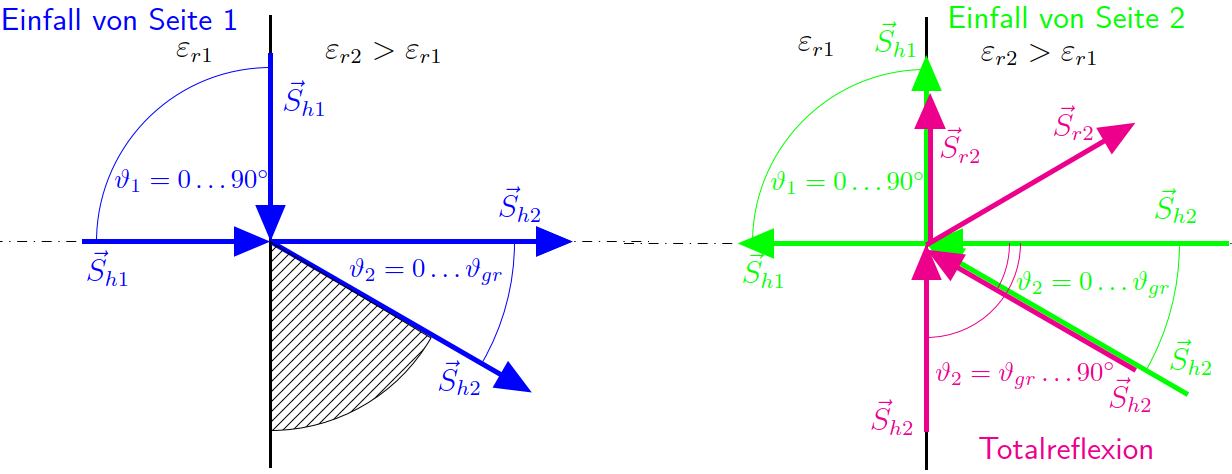
\includegraphics[width=\columnwidth]{Figures/Grenzwinkel_Bild.png}

\subsubsection[Brewster-/Polarisationswinkel]{Brewster-/Polarisationswinkel}
Bei Brewster-Winkel $ \theta_b $ wird Reflexionsfaktor $r=0$.
\begin{itemize}
	%    \item Snelliusche Brechungsgesetz
	%\item Grenzwinkel $\alpha_g$
	% \item[--] Brewsterwinkel $\alpha_B$ (Welle transmittiert reflexionsfrei)
	%       \begin{itemize}
		%           \item[\textbullet] Parallele Polarisation (Nur wenn $\mu_{r1} = \mu_{r2}$)
		%           \item[\textbullet] Senkrechte Polarisation (Nur wenn $\varepsilon_{r1} = \varepsilon_{r2}$)
		%       \end{itemize}
	\item \textbf{Parallele} Polarisation: \quad rechts:
	$ \mu_{r1}=\mu_{r2} $
	\begin{align*}
%		\Aboxed{\mu_{r1}=\mu_{r2}}\\
		\sin\theta_b & = \sqrt{\frac{\varepsilon_2(\mu_2\varepsilon_1 - \mu_1\varepsilon_2)}{\mu_1(\varepsilon_1^2-\varepsilon_2^2)}} &
		\Aboxed{\tan\theta_b & = \sqrt{\frac{\varepsilon_2}{\varepsilon_1}} = \frac{n_2}{n_1}}&
	\end{align*}
		Brewster-Winkel existiert nur bei $ \varepsilon_{r1} \neq \varepsilon_{r2} $.
    \item \textbf{Senkrechte} Polarisation:  \quad rechts: $ \varepsilon_{r1} = \varepsilon_{r2} $
	\begin{align*}
%		\Aboxed{\varepsilon_{r1}=\varepsilon_{r2}}         \\
		\sin\theta_b & = \sqrt{\frac{\mu_2(\mu_2\varepsilon_1 - \mu_1\varepsilon_2)}{\varepsilon_1(\mu_2^2-\mu_1^2)}}&
		\tan\theta_b & = \sqrt{\frac{\mu_2}{\mu_1+\mu_2}}&
	\end{align*}
	Brewster-Winkel existiert nur bei $ \mu_{r1} \neq \mu_{r2} $.\\
	Bei $ \mu_{r1}=\mu_{r2} \rightarrow r \neq 0$ keine Reflexionsfreiheit!
\end{itemize}

\subsubsection{Verlauf von r und t beim Grenzübergang}
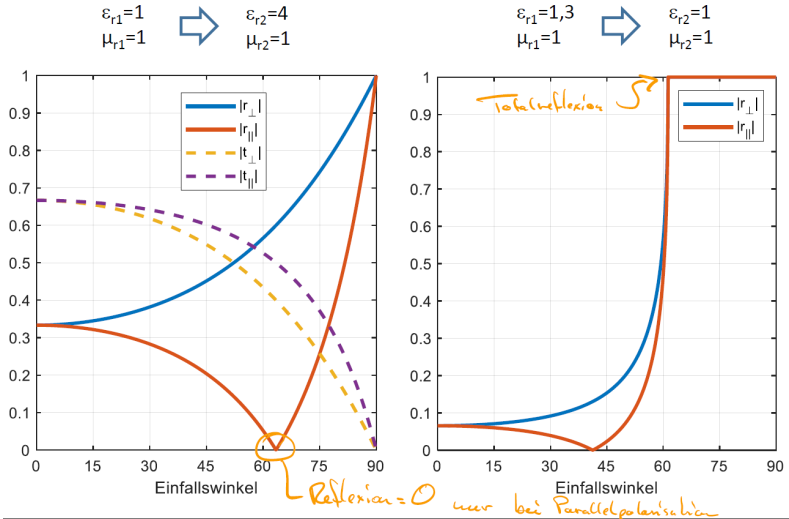
\includegraphics[width=\columnwidth]{Figures/Totalreflexion_Diagramm.png}

\subsubsection{Verlauf der Reflexionsfaktoren}
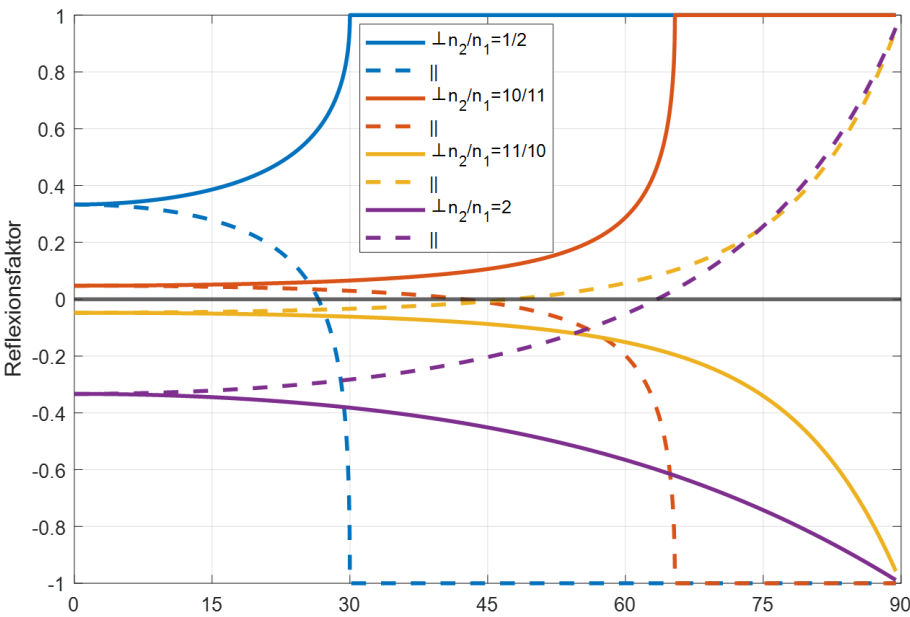
\includegraphics[width=\columnwidth]{Figures/Verlauf_Reflexionsfaktoren.png}

\newpage
\subsection{Senkrechte (E-Feld) Polarisation (H-Feld parallel)}
\begin{center}
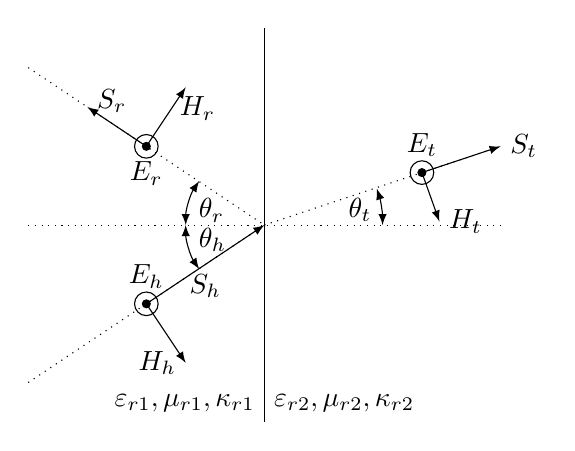
\begin{tikzpicture}
	\tikzset{cross/.style={cross out, draw=black, minimum size=2*(#1-\pgflinewidth), inner sep=0pt, outer sep=0pt},
		%     %default radius will be 1pt. 
		cross/.default={3.5pt}}
	%Kreuz
	\draw[dotted] (-3,0) -- (3,0);
	\draw[-] (0,2.5) -- (0,-2.5)                
	node[above right]   {$\varepsilon_{r2}, \mu_{r2}, \kappa_{r2}$}
	node[above left]    {$\varepsilon_{r1}, \mu_{r1}, \kappa_{r1}$};
	%Rücklaufende
	\draw[-latex] (-1.5,1) -- (-2.25,1.5)   node[right, yshift=.5ex]{$S_r$};
	\draw[-latex] (-1.5,1) -- (-1,1.75)     node[below, xshift=1ex] {$H_r$};
	\draw[-] (-1.5,1) circle (0.15)         node[below,yshift=-.5ex]{$E_r$};
	\draw[-,fill=black!100] (-1.5,1) circle (0.05);
	\draw[dotted] (-3,2) -- (0,0);
	\draw[latex-latex] (146:1) arc (146:180:1) 
	node[midway, right, yshift=-.7ex] {$\theta_r$};
	
	%Hinlaufende
	\draw[-latex] (-1.5,-1) -- (0,0)        node[below, midway]         {$S_h$};
	\draw[-latex] (-1.5,-1) -- (-1,-1.75)   node[left]                  {$H_h$};
	\draw[-] (-1.5,-1) circle (0.15)        node[above, yshift=.5ex]    {$E_h$};
	\draw[-,fill=black!100] (-1.5,-1) circle (0.05);
	\draw[dotted] (-3,-2) -- (0,0);
	\draw[latex-latex] (180:1) arc (180:214:1)
	node[midway, right, yshift=.7ex] {$\theta_h$};
	
	%Transmitierte
	\draw[-latex] (2,0.6666) -- (3,1)           node[right] {$S_t$};
	\draw[-latex] (2,0.6666) -- (2.2223,0.0448) node[right] {$H_t$};
	\draw[-] (2,0.6666) circle (0.15)           node[above, yshift=.5ex] {$E_t$};
	\draw[-,fill=black!100] (2,0.6666) circle (0.05);
	\draw[dotted] (0,0) -- (3,1);
	\draw[latex-latex] (0:1.5) arc (0:18:1.5)
	node[midway, left, yshift=-.3ex] {$\theta_t$};
	
\end{tikzpicture}
\end{center}



\[ \boxed{\texttt{mit } Z_{F0} = 120\pi \approx 377\si{\ohm}} \]
\begin{align*}
    Z_{Fn}                & = Z_{F0}\cdot\frac{1}{\sqrt{\varepsilon_{rn}}}            \\
    \frac{Z_{F1}}{Z_{F2}} & = \frac{\sqrt{\varepsilon_{r2}}}{\sqrt{\varepsilon_{r1}}}
\end{align*}
\[ n: \texttt{Brechungsindex} \quad ; \quad \theta_h = \theta_r\]
\begin{align*}
    \frac{\sin\theta_t}{\sin\theta_h} & = \frac{\lambda_2}{\lambda_1}= \frac{\beta_1}{\beta_2}= \frac{n_1}{n_2} \\
    \sin\theta_t                      & = \sqrt{\frac{\varepsilon_{r1}}{\varepsilon_{r2}}}\cdot \sin\theta_h
\end{align*}

\begin{itemize}
    \item magnetischer/elektrischer Reflexionsfaktor $[1]$
    \item magnetischer Transmissionsfaktor $[1]$
    \item elektrischer Transmissionsfaktor $[1]$
\end{itemize}
\begin{align*}
    r_s    & =  r_{es} = r_{ms} =                                                                                                                                            \\
           & = \frac{Z_{F2} \cdot \cos \theta_h-Z_{F1} \cdot \cos \theta_t}{Z_{F2} \cdot \cos \theta_h+Z_{F1} \cdot \cos \theta_t}                                           \\
           & = \frac{\cos\theta_h-\sqrt{^{\varepsilon_{r2}}/_{\varepsilon_{r1}}-\sin^2\theta_h}}{\cos\theta_h+\sqrt{^{\varepsilon_{r2}}/_{\varepsilon_{r1}}-\sin^2\theta_h}} \\
    t_{ms} & = Z_{F1} \cdot \frac{2 \cdot \cos \theta_h}{Z_{F2} \cdot \cos \theta_h+Z_{F1} \cdot \cos \theta_t}                                                              \\
           & = (1 - r_s) \cdot \dfrac{\cos \theta_h}{\cos \theta_t}                                                                                                          \\
           & = \frac{Z_{F1}}{Z_{F2}}\cdot t_{es}                                                                                                                             \\
    t_{es} & = Z_{F2} \cdot \frac{2 \cdot \cos \theta_h}{Z_{F2} \cdot \cos \theta_h+Z_{F1} \cdot \cos \theta_t}                                                              \\
           & = 1+r_s
\end{align*}

\begin{align*}
    E_r & = r_s \cdot E_h    \\
    E_t & = t_{es} \cdot E_h \\
    H_r & = r_s \cdot H_h    \\
    H_t & = t_{ms} \cdot H_h \\
    E_t & = H_t\cdot Z_{F2}  \\
    E_h & = H_h\cdot Z_{F1}
\end{align*}

\subsection{Parallel (E-Feld) Polarisation (H-Feld senkrecht)}
\begin{tikzpicture}
    \tikzset{cross/.style={cross out, draw=black, minimum size=2*(#1-\pgflinewidth), inner sep=0pt, outer sep=0pt},
        %     %default radius will be 1pt. 
        cross/.default={3.5pt}}
    %Kreunz
    \draw[dotted] (-3,0) -- (3,0);
    \draw[-] (0, 2.5) -- (0,-2.5) node[above right] {$\varepsilon_{r2}, \mu_{r2}, \kappa_{r2}$}
        node[above left] {$\varepsilon_{r1}, \mu_{r1}, \kappa_{r1}$};
 
    %Hinlaufende
    \draw[-latex] (-1.5,-1) -- (0,0) node[below, midway ]       {$S_h$};
    \draw[-latex] (-1.5,-1) -- (-2,-0.25) node[left, midway]    {$E_h$};
    \draw[-] (-1.5,-1) circle (0.15) node[below,yshift=-.5ex]   {$H_h$};
    \draw[-,fill=black!100] (-1.5,-1) circle (0.05);
    \draw[dotted] (-3,-2) -- (0,0);
    \draw[latex-latex] (180:1) arc (180:214:1)
        node[midway, right, yshift=.7ex] {$\theta_h$};

    %Rücklaufende
    \draw[-latex] (-1.5,1) -- (-2.25,1.5) node[right, yshift=.5ex]          {$S_r$};
    \draw[-latex] (-1.5,1) -- (-2,0.25) node[left, yshift=1ex, xshift=1ex]  {$E_r$};
    \draw[-] (-1.5,1) circle (0.15) node[above, yshift=.5ex]                {$H_r$};
    \draw[-,fill=black!100] (-1.5,1) circle (0.05);
    \draw[dotted] (-3,2) -- (0,0);
    \draw[latex-latex] (146:1) arc (146:180:1)
        node[midway, right, yshift=-.7ex] {$\theta_r$};
        
%    Rücklaufende Sattler
	%    Rücklaufende Sattler
	\draw[-] (-0.8,1.2) circle (0.15) node[right, xshift=.5ex]                {$H_r$};
	\draw(-0.8,1.2) node [cross] {};
 	\draw[-latex] (-0.8,1.2) -- (-0.3,1.95) node[left, yshift=1ex, xshift=1ex]  {$E_r$};
  	\draw[-latex] (-0.8,1.2) -- (-1.55,1.7) node[right, yshift=.5ex]          {$S_r$};

    %Transmitierte
    \draw[-latex] (2,0.6666) -- (3,1) node[right]                   {$S_t$};
    \draw[-latex] (2,0.6666) -- (1.7777,1.378)  node[right]         {$E_t$};
    \draw[-] (2,0.6666) circle (0.15) node[below, yshift=-0.5ex]    {$H_t$};
    \draw[-,fill=black!100] (2,0.6666) circle (0.05);
    \draw[dotted] (0,0) -- (3,1);
    \draw[latex-latex] (0:1.5) arc (0:18:1.5)
        node[midway, left, yshift=-.7] {$\theta_t$};

\end{tikzpicture}

\[ \boxed{\texttt{mit } Z_{F0} = 120\pi \approx 377\si{\ohm}} \]
\begin{align*}
    Z_{Fn}                & = Z_{F0}\cdot\frac{1}{\sqrt{\varepsilon_{rn}}}            \\
    \frac{Z_{F1}}{Z_{F2}} & = \frac{\sqrt{\varepsilon_{r2}}}{\sqrt{\varepsilon_{r1}}}
\end{align*}
\[ n: \texttt{Brechungsindex} \quad ; \quad \theta_h = \theta_r\]
\begin{align*}
    \frac{\sin\theta_t}{\sin\theta_h} & = \frac{\lambda_2}{\lambda_1}= \frac{\beta_1}{\beta_2}= \frac{n_1}{n_2} \\
    \sin\theta_t                      & = \sqrt{\frac{\varepsilon_{r1}}{\varepsilon_{r2}}}\cdot\sin\theta_h
\end{align*}

\begin{itemize}
    \item magnetischer/elektrischer Reflexionsfaktor $[1]$
    \item magnetischer Transmissionsfaktor $[1]$
    \item elektrischer Transmissionsfaktor $[1]$
\end{itemize}
\begin{align*}
    r_p    & =  r_{ep} = r_{mp} =                                                                                                                                                                                                        \\
           & = \frac{Z_{F2} \cdot \cos \theta_t-Z_{F1} \cdot \cos \theta_h}{Z_{F2} \cdot \cos \theta_t+Z_{F1} \cdot \cos \theta_h} =                                                                                                     \\
           & = \frac{\varepsilon_{r2}\cos\theta_h-\sqrt{\varepsilon_{r2}\varepsilon_{r1}-{\varepsilon_{r1}}^2\sin^2\theta_h}}{\varepsilon_{r2}\cos\theta_h+\sqrt{{\varepsilon_{r2}\varepsilon_{r1}-{\varepsilon_{r1}}^2\sin^2\theta_h}}} \\
    t_{mp} & = Z_{F1} \cdot \frac{2 \cdot \cos \theta_h}{Z_{F1} \cdot \cos \theta_h+Z_{F2} \cdot \cos \theta_t}                                                                                                                          \\
           & = 1+r_p                                                                                                                                                                                                                     \\
    t_{ep} & = Z_{F2} \cdot \frac{2 \cdot \cos \theta_h}{Z_{F1} \cdot \cos \theta_h+Z_{F2} \cdot \cos \theta_t}                                                                                                                          \\
           & = (1-r_p) \cdot \dfrac{\cos \theta_h}{\cos \theta_t}                                                                                                                                                                        \\
           & = \frac{Z_{F2}}{Z_{F1}}\cdot t_{mp}
\end{align*}

\begin{align*}
    E_r & = r_p\cdot E_h    \\
    E_t & = t_{ep}\cdot E_h \\
    H_r & = r_p\cdot H_h    \\
    H_t & = t_{mp}\cdot H_h \\
    E_t & = H_t\cdot Z_{F2} \\
    E_h & = H_h\cdot Z_{F1}
\end{align*}

\newpage
\subsubsection{Senkrechte Polarisation mit $\mu_r$}
\begin{center}
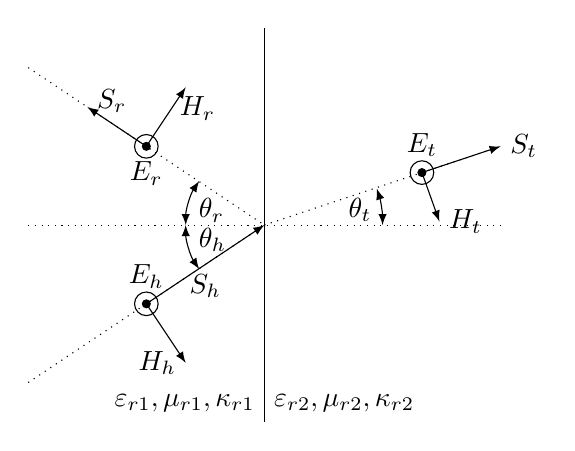
\begin{tikzpicture}
	\tikzset{cross/.style={cross out, draw=black, minimum size=2*(#1-\pgflinewidth), inner sep=0pt, outer sep=0pt},
		%     %default radius will be 1pt. 
		cross/.default={3.5pt}}
	%Kreuz
	\draw[dotted] (-3,0) -- (3,0);
	\draw[-] (0,2.5) -- (0,-2.5)                
	node[above right]   {$\varepsilon_{r2}, \mu_{r2}, \kappa_{r2}$}
	node[above left]    {$\varepsilon_{r1}, \mu_{r1}, \kappa_{r1}$};
	%Rücklaufende
	\draw[-latex] (-1.5,1) -- (-2.25,1.5)   node[right, yshift=.5ex]{$S_r$};
	\draw[-latex] (-1.5,1) -- (-1,1.75)     node[below, xshift=1ex] {$H_r$};
	\draw[-] (-1.5,1) circle (0.15)         node[below,yshift=-.5ex]{$E_r$};
	\draw[-,fill=black!100] (-1.5,1) circle (0.05);
	\draw[dotted] (-3,2) -- (0,0);
	\draw[latex-latex] (146:1) arc (146:180:1) 
	node[midway, right, yshift=-.7ex] {$\theta_r$};
	
	%Hinlaufende
	\draw[-latex] (-1.5,-1) -- (0,0)        node[below, midway]         {$S_h$};
	\draw[-latex] (-1.5,-1) -- (-1,-1.75)   node[left]                  {$H_h$};
	\draw[-] (-1.5,-1) circle (0.15)        node[above, yshift=.5ex]    {$E_h$};
	\draw[-,fill=black!100] (-1.5,-1) circle (0.05);
	\draw[dotted] (-3,-2) -- (0,0);
	\draw[latex-latex] (180:1) arc (180:214:1)
	node[midway, right, yshift=.7ex] {$\theta_h$};
	
	%Transmitierte
	\draw[-latex] (2,0.6666) -- (3,1)           node[right] {$S_t$};
	\draw[-latex] (2,0.6666) -- (2.2223,0.0448) node[right] {$H_t$};
	\draw[-] (2,0.6666) circle (0.15)           node[above, yshift=.5ex] {$E_t$};
	\draw[-,fill=black!100] (2,0.6666) circle (0.05);
	\draw[dotted] (0,0) -- (3,1);
	\draw[latex-latex] (0:1.5) arc (0:18:1.5)
	node[midway, left, yshift=-.3ex] {$\theta_t$};
	
\end{tikzpicture}
\end{center}


$\vec{E}$-Feld senkrecht, $ \vec{H}$-Feld parallel. \qquad $ \mu_{r1} \neq \mu_{r2} $
%\[ \boxed{\texttt{mit } Z_{F0} = 120\pi \approx 377\si{\ohm}} \]
\begin{flalign*}
	Z_{F0} &= 120\pi \,\si{\ohm} &
	Z_{F(n)}                & = Z_{F0}\cdot\sqrt{\frac{\mu_{r(n)}}{\varepsilon_{r(n)}}}&
	\frac{Z_{F1}}{Z_{F2}} & = \frac{\sqrt{\mu_{r 1}\varepsilon_{r2}}}{\sqrt{\mu_{r 2}\varepsilon_{r1}}}&
\end{flalign*}
%\[ n: \texttt{Brechungsindex} \quad ; \quad \theta_h = \theta_r\]
\textbf{Brechungsgesetz}: \qquad  mit $ \theta_h = \theta_r\ $
\begin{flalign*}
	\Aboxed{\frac{\sin\theta_t}{\sin\theta_h} & = \sqrt{\frac{\mu_{r 1}\varepsilon_{r1}}{\mu_{r 2}\varepsilon_{r2}}}} = \frac{\lambda_2}{\lambda_1}= \frac{\beta_1}{\beta_2}= \frac{n_1}{n_2} &
%	\sin\theta_t                      & = \sqrt{\frac{\varepsilon_{r1}}{\varepsilon_{r2}}}\cdot \sin\theta_h 
\end{flalign*}
%\begin{align*}
%	\dfrac{\sin \vartheta_{2}}{\sin \vartheta_{1}} = \dfrac{k_{h}}{k_{g}} & = \sqrt{\dfrac{\mu_{r 1} \varepsilon_{r 1}}{\mu_{r 2} \varepsilon_{r 2}}} = \dfrac{n_{1}}{n_{2}} = \dfrac{v_{p, 2}}{v_{p, 1}} = \dfrac{\lambda_{2}}{\lambda_{1}} \\
%	% \alpha_{Bp}                                                           & = \tan^{-1} \left( \sqrt{ \dfrac{\varepsilon_{r1}}{\varepsilon_{r2}}} \right)                                                                                        \\
%	% \alpha_{Bs}                                                           & = \tan^{-1} \left( \sqrt{ \dfrac{\mu_{r1}}{\mu_{r2}}} \right)
%\end{align*}


%\begin{itemize}
%    \item magnetischer/elektrischer Reflexionsfaktor $[1]$
%    \item magnetischer Transmissionsfaktor $[1]$
%    \item elektrischer Transmissionsfaktor $[1]$
%\end{itemize}
\textbf{Fresnelsche Formeln}: \qquad $ \theta_h = \vartheta_{1} $ \quad $ \theta_t = \vartheta_{2} $
\begin{equation*}
	\setlength{\jot}{10pt}
	\begin{aligned}
		r_s    & =  r_{es} = r_{ms} =                                                                                                                                            \\
		& = \frac{Z_{F2} \cdot \cos \theta_h-Z_{F1} \cdot \cos \theta_t}{Z_{F2} \cdot \cos \theta_h+Z_{F1} \cdot \cos \theta_t}                                           \\
		%		& = \frac{\cos\theta_h-\sqrt{^{\varepsilon_{r2}}/_{\varepsilon_{r1}}-\sin^2\theta_h}}{\cos\theta_h+\sqrt{^{\varepsilon_{r2}}/_{\varepsilon_{r1}}-\sin^2\theta_h}} \\
& =\frac{\cos \vartheta_1-\sqrt{\frac{\mu_{r 1} \varepsilon_{r 2}}{\mu_{r 2} \varepsilon_{r 1}}-\frac{\mu_{r 1}{ }^2}{\mu_{r 2}^2} \sin ^2 \vartheta_1}}{\cos \vartheta_1+\sqrt{\frac{\mu_{r 1} \varepsilon_{r 2}}{\mu_{r 2} \varepsilon_{r 1}}-\frac{\mu_{r 1}{ }^2}{\mu_{r 2}^2} \sin ^2 \vartheta_1}} \\
		t_{es} & =\frac{2 \cdot	 Z_{F2} \cdot \cos \theta_h}{Z_{F2} \cdot \cos \theta_h+Z_{F1} \cdot \cos \theta_t}                                                              \\
& =\frac{2 \cos \vartheta_1}{\cos \vartheta_1+\sqrt{\frac{\mu_{r 1} \varepsilon_{r 2}}{\mu_{r 2} \varepsilon_{r 1}}-\frac{\mu_{r 1}{ }^2}{\mu_{r 2}{ }^2} \sin ^2 \vartheta_1}} \\
		& = 1+r_s\\
		t_{ms} & = \frac{2 Z_{F1} \cdot \cos \theta_h}{Z_{F2} \cdot \cos \theta_h+Z_{F1} \cdot \cos \theta_t}                                                              \\
		& =\frac{2 \sqrt{\frac{\mu_{r 1} \varepsilon_{r 2}}{\mu_{r 2} \varepsilon_{r 1}}} \cos \vartheta_1}{\cos \vartheta_1+\sqrt{\frac{\mu_{r 1} \varepsilon_{r 2}}{\mu_{r 2} \varepsilon_{r 1}}-\frac{\mu_{r 1}{ }^2}{\mu_{r 2}{ }^2} \sin ^2 \vartheta_1}}
		\\
%		& = (1 - r_s) \cdot \dfrac{\cos \theta_h}{\cos \theta_t}                                                                                                          \\
		& = \frac{Z_{F1}}{Z_{F2}}\cdot t_{es}\\
		& =\sqrt{\frac{\mu_{r 1} \varepsilon_{r 2}}{\mu_{r 2} \varepsilon_{r 1}}} t_{e s}                                                                                                                   
	\end{aligned}
\end{equation*}


%\begin{align*}
%    r_s    & =  r_{es} = r_{ms} =                                                                                                                                            \\
%           & = \frac{Z_{F2} \cdot \cos \theta_h-Z_{F1} \cdot \cos \theta_t}{Z_{F2} \cdot \cos \theta_h+Z_{F1} \cdot \cos \theta_t}                                           \\
%           & = \frac{\cos\theta_h-\sqrt{^{\varepsilon_{r2}}/_{\varepsilon_{r1}}-\sin^2\theta_h}}{\cos\theta_h+\sqrt{^{\varepsilon_{r2}}/_{\varepsilon_{r1}}-\sin^2\theta_h}} \\
%           & = \frac{\sqrt{\varepsilon_{r1}}\cdot\cos\theta_h - \sqrt{\varepsilon_{r2}}\cdot\cos\theta_t}{\sqrt{\varepsilon_{r2}}\cdot\cos\theta_t + \sqrt{\varepsilon_{r1}}\cos\theta_h} \\
%    t_{ms} & = Z_{F1} \cdot \frac{2 \cdot \cos \theta_h}{Z_{F2} \cdot \cos \theta_h+Z_{F1} \cdot \cos \theta_t}                                                              \\
%           & = (1 - r_s) \cdot \dfrac{\cos \theta_h}{\cos \theta_t}                                                                                                          \\
%           & = \frac{Z_{F1}}{Z_{F2}}\cdot t_{es}                                                                                                                             \\
%    t_{es} & = Z_{F2} \cdot \frac{2 \cdot \cos \theta_h}{Z_{F2} \cdot \cos \theta_h+Z_{F1} \cdot \cos \theta_t}                                                              \\
%           & = 1+r_s
%\end{align*}
%\subsubsection*{Beziehungen Polarisation}
%\textbf{Beziehungen Polarisation}
%\begin{equation*}
%	\begin{aligned}
%		E_r & = r_s \cdot E_h    \\
%		E_t & = t_{es} \cdot E_h \\
%		H_r & = r_s \cdot H_h    \\
%		H_t & = t_{ms} \cdot H_h \\
%		E_t & = H_t\cdot Z_{F2}  \\
%		E_h & = H_h\cdot Z_{F1}
%	\end{aligned}
%	\qquad
%	\begin{aligned}
%		E_r & = r_p\cdot E_h    \\
%		E_t & = t_{ep}\cdot E_h \\
%		H_r & = r_p\cdot H_h    \\
%		H_t & = t_{mp}\cdot H_h \\
%		E_t & = H_t\cdot Z_{F2} \\
%		E_h & = H_h\cdot Z_{F1} 
%	\end{aligned}
%\end{equation*}
%
%\textbf{Richtungssinn Felder (Hand-Regel)}
%\begin{equation*}
%	\begin{aligned}
%		& \text{\textbf{Linke Hand}}\\
%		& \text{Daumen:}\quad \vec{E}\\
%		& \text{Zeigef.:}\quad \vec{S}_{av}\\
%		& \text{Mittelf.:}\quad \vec{H} 
%	\end{aligned}
%	\qquad
%	\begin{aligned}
%		& \text{\textbf{Rechte Hand}}\\
%		& \text{Daumen:}\quad \vec{E}\\
%		& \text{Zeigef.:}\quad \vec{H}\\
%		& \text{Mittelf.:}\quad \vec{S}_{av}
%	\end{aligned}
%\end{equation*}
\newcolumn
\subsubsection{Parallele Polarisation mit $\mu_r$}
\begin{center}
	\begin{tikzpicture}
    \tikzset{cross/.style={cross out, draw=black, minimum size=2*(#1-\pgflinewidth), inner sep=0pt, outer sep=0pt},
        %     %default radius will be 1pt. 
        cross/.default={3.5pt}}
    %Kreunz
    \draw[dotted] (-3,0) -- (3,0);
    \draw[-] (0, 2.5) -- (0,-2.5) node[above right] {$\varepsilon_{r2}, \mu_{r2}, \kappa_{r2}$}
        node[above left] {$\varepsilon_{r1}, \mu_{r1}, \kappa_{r1}$};
 
    %Hinlaufende
    \draw[-latex] (-1.5,-1) -- (0,0) node[below, midway ]       {$S_h$};
    \draw[-latex] (-1.5,-1) -- (-2,-0.25) node[left, midway]    {$E_h$};
    \draw[-] (-1.5,-1) circle (0.15) node[below,yshift=-.5ex]   {$H_h$};
    \draw[-,fill=black!100] (-1.5,-1) circle (0.05);
    \draw[dotted] (-3,-2) -- (0,0);
    \draw[latex-latex] (180:1) arc (180:214:1)
        node[midway, right, yshift=.7ex] {$\theta_h$};

    %Rücklaufende
    \draw[-latex] (-1.5,1) -- (-2.25,1.5) node[right, yshift=.5ex]          {$S_r$};
    \draw[-latex] (-1.5,1) -- (-2,0.25) node[left, yshift=1ex, xshift=1ex]  {$E_r$};
    \draw[-] (-1.5,1) circle (0.15) node[above, yshift=.5ex]                {$H_r$};
    \draw[-,fill=black!100] (-1.5,1) circle (0.05);
    \draw[dotted] (-3,2) -- (0,0);
    \draw[latex-latex] (146:1) arc (146:180:1)
        node[midway, right, yshift=-.7ex] {$\theta_r$};
        
%    Rücklaufende Sattler
	%    Rücklaufende Sattler
	\draw[-] (-0.8,1.2) circle (0.15) node[right, xshift=.5ex]                {$H_r$};
	\draw(-0.8,1.2) node [cross] {};
 	\draw[-latex] (-0.8,1.2) -- (-0.3,1.95) node[left, yshift=1ex, xshift=1ex]  {$E_r$};
  	\draw[-latex] (-0.8,1.2) -- (-1.55,1.7) node[right, yshift=.5ex]          {$S_r$};

    %Transmitierte
    \draw[-latex] (2,0.6666) -- (3,1) node[right]                   {$S_t$};
    \draw[-latex] (2,0.6666) -- (1.7777,1.378)  node[right]         {$E_t$};
    \draw[-] (2,0.6666) circle (0.15) node[below, yshift=-0.5ex]    {$H_t$};
    \draw[-,fill=black!100] (2,0.6666) circle (0.05);
    \draw[dotted] (0,0) -- (3,1);
    \draw[latex-latex] (0:1.5) arc (0:18:1.5)
        node[midway, left, yshift=-.7] {$\theta_t$};

\end{tikzpicture}
\end{center}
$\vec{E}$-Feld parallel, $ \vec{H}$-Feld senkrecht. \qquad $ \mu_{r1} \neq \mu_{r2} $\\

Stücke: $\vec{H}_h$ und $ \vec{H}_r$ zeigen in die selbe Richtung!\\
Sattler: $\vec{H}_h$ und $ \vec{H}_r$ zeigen in \textbf{entgegengesetzter} Richtung!\\
%\[ \boxed{\texttt{mit } Z_{F0} = 120\pi \approx 377\si{\ohm}} \]
%\begin{align*}
%    Z_{Fn}                & = Z_{F0}\cdot\frac{1}{\sqrt{\varepsilon_{rn}}}            \\
%    \frac{Z_{F1}}{Z_{F2}} & = \frac{\sqrt{\varepsilon_{r2}}}{\sqrt{\varepsilon_{r1}}}
%\end{align*}
%\[ n: \texttt{Brechungsindex} \quad ; \quad \theta_h = \theta_r\]
%\begin{align*}
%    \frac{\sin\theta_t}{\sin\theta_h} & = \frac{\lambda_2}{\lambda_1}= \frac{\beta_1}{\beta_2}= \frac{n_1}{n_2} \\
%    \sin\theta_t                      & = \sqrt{\frac{\varepsilon_{r1}}{\varepsilon_{r2}}}\cdot\sin\theta_h
%\end{align*}

%\begin{itemize}
%    \item magnetischer/elektrischer Reflexionsfaktor $[1]$
%    \item magnetischer Transmissionsfaktor $[1]$
%    \item elektrischer Transmissionsfaktor $[1]$
%\end{itemize}
\textbf{Fresnelsche Formeln (Stücke)}: \qquad $ \theta_h = \vartheta_{1} $ \quad $ \theta_t = \vartheta_{2} $
\begin{equation*}
	\setlength{\jot}{10pt}
	\begin{aligned}
		r_{ep}    & =  r_{mp} = r_{p}  \qquad \qquad =-r_{p,[\texttt{Sattler}]}
		\\
		& = \frac{Z_{F1} \cdot \cos \theta_h-Z_{F2} \cdot \cos \theta_t}{Z_{F1} \cdot \cos \theta_h+Z_{F2} \cdot \cos \theta_t}
		\\
		%		& = - \left( \frac{\varepsilon_{r2}\cos\theta_h-\sqrt{\varepsilon_{r2}\varepsilon_{r1}-{\varepsilon_{r1}}^2\sin^2\theta_h}}{\varepsilon_{r2}\cos\theta_h+\sqrt{{\varepsilon_{r2}\varepsilon_{r1}-{\varepsilon_{r1}}^2\sin^2\theta_h}}} \right)  
		%		\\
%		& =\frac{\cos \vartheta_1-\sqrt{\frac{\varepsilon_{r 1}}{\varepsilon_{r 2}}-\frac{\varepsilon_{r 1}{ }^2}{\varepsilon_{r 2}{ }^2} \sin ^2 \vartheta_1}}{\cos \vartheta_1+\sqrt{\frac{\varepsilon_{r 1}}{\varepsilon_{r 2}}-\frac{\varepsilon_{r 1}{ }^2}{\varepsilon_{r 2}{ }^2} \sin ^2 \vartheta_1}}
%		\\
		& =\frac{\cos \vartheta_1-\sqrt{\frac{\mu_{r 2} \varepsilon_{r 1}}{\mu_{r 1} \varepsilon_{r 2}}-\frac{\varepsilon_{r 1}{ }^2}{\varepsilon_{r 2}{ }^2} \sin ^2 \vartheta_1}}{\cos \vartheta_1+\sqrt{\frac{\mu_{r 2} \varepsilon_{r 1}}{\mu_{r 1} \varepsilon_{r 2}}-\frac{\varepsilon_{r 1}{ }^2}{\varepsilon_{r 2}{} ^2} \sin ^2 \vartheta_1}} \\
		t_{ep} & =  \frac{2 \cdot Z_{F2}   \cdot  \cos \theta_h}{Z_{F1} \cdot \cos \theta_h+Z_{F2} \cdot \cos \theta_t}\\                                                                                                                           %= (1-r_p) \cdot \dfrac{\cos \theta_h}{\cos \theta_t}                                                                                                                                                                        \\
				&=\frac{2 \sqrt{\frac{\mu_{r 2} \varepsilon_{r 1}}{\mu_{r 1} \varepsilon_{r 2}}} \cos \vartheta_1}{\cos \vartheta_1+\sqrt{\frac{\mu_{r 2} \varepsilon_{r 1}}{\mu_{r 1} \varepsilon_{r 2}}-\frac{\varepsilon_{r 1}{ }^2}{\varepsilon_{r 2}{ }^2} \sin ^2 \vartheta_1}} \\
%		& = \frac{2 \sqrt{\frac{\varepsilon_{r 1}}{\varepsilon_{r 2}}} \cos \vartheta_1}{\cos \vartheta_1+\sqrt{\frac{\varepsilon_{r 1}}{\varepsilon_{r 2}}-\frac{\varepsilon_{r 1}^2}{\varepsilon_{r 2}{ }^2} \sin ^2 \vartheta_1}}
%		\\
		& = \frac{Z_{F2}}{Z_{F1}}\cdot t_{mp} = \sqrt{\frac{\mu_{r2}\varepsilon_{r1}}{\mu_{r1}\varepsilon_{r2}}}\cdot t_{mp} 
		\\
		t_{mp} & = \frac{2 \cdot  Z_{F1}\cdot \cos \theta_h}{Z_{F1} \cdot \cos \theta_h+Z_{F2} \cdot \cos \theta_t}                    
\\
		&=\frac{2 \cos \vartheta_1}{\cos \vartheta_1+\sqrt{\frac{\mu_{r 2} \varepsilon_{r 1}}{\mu_{r 1} \varepsilon_{r 2}}-\frac{\varepsilon_{r 1}{ }^2}{\varepsilon_{r 2}{ }^2} \sin ^2 \vartheta_1}}   \\
		&		= 1+r_p
	\end{aligned}
\end{equation*}
%\begin{align*}
%    r_p    & =  r_{ep} = r_{mp} =                                                                                                                                                                                                        \\
%           & = \frac{Z_{F1} \cdot \cos \theta_t-Z_{F2} \cdot \cos \theta_h}{Z_{F2} \cdot \cos \theta_t+Z_{F1} \cdot \cos \theta_h} =                                                                                                     \\
%           & = \frac{\varepsilon_{r2}\cos\theta_h-\sqrt{\varepsilon_{r2}\varepsilon_{r1}-{\varepsilon_{r1}}^2\sin^2\theta_h}}{\varepsilon_{r2}\cos\theta_h+\sqrt{{\varepsilon_{r2}\varepsilon_{r1}-{\varepsilon_{r1}}^2\sin^2\theta_h}}} \\
%               t_{ep} & = Z_{F2} \cdot \frac{2 \cdot \cos \theta_h}{Z_{F1} \cdot \cos \theta_h+Z_{F2} \cdot \cos \theta_t}                                                                                                                          \\
%           & = (1-r_p) \cdot \dfrac{\cos \theta_h}{\cos \theta_t}                                                                                                                                                                        \\
%           & = \frac{Z_{F2}}{Z_{F1}}\cdot t_{mp}\\
%    t_{mp} & = \frac{2 Z_{F1}\cdot \cos \theta_h}{Z_{F1} \cdot \cos \theta_h+Z_{F2} \cdot \cos \theta_t}                                                                                                                          \\
%           & = 1+r_p                                                                                                                                                                                                                
%\end{align*}
%\textbf{Fresnelsche Formeln (Sattler)}:
%\begin{equation*}
%	\setlength{\jot}{10pt}
%	\begin{aligned}
%		r_p    & =  r_{ep} = r_{mp} \qquad \qquad =-r_{p,[\texttt{Stücke}]}                                                    \\
%		& = \frac{Z_{F2} \cdot \cos \theta_t-Z_{F1} \cdot \cos \theta_h}{Z_{F2} \cdot \cos \theta_t+Z_{F1} \cdot \cos \theta_h}                                                                                               \\
%		& = \frac{\sqrt{\varepsilon_{r1}}\cdot\cos\theta_t - \sqrt{\varepsilon_{r2}}\cdot\cos\theta_h}{\sqrt{\varepsilon_{r2}}\cdot\cos\theta_h + \sqrt{\varepsilon_{r1}}\cos\theta_t} \\
%		t_{ep} & =  \frac{2 Z_{F2} \cdot \cos \theta_h}{Z_{F1} \cdot \cos \theta_h+Z_{F2} \cdot \cos \theta_t}                                                                                                                          \\
%		& = \frac{2\cdot\sqrt{\varepsilon_{r1}}\cdot\cos\theta_h}{\sqrt{\varepsilon_{r2}}\cdot\cos\theta_h + \sqrt{\varepsilon_{r1}}\cdot\cos\theta_t}\\
%		& = (1+r_p) \cdot \dfrac{\cos \theta_h}{\cos \theta_t}\\
%		t_{mp} 
%		%	& 
%		%	= \frac{2 Z_{F1}\cdot \cos \theta_h}{Z_{F1} \cdot \cos \theta_h+Z_{F2} \cdot \cos \theta_t}                                                                                                                          \\
%		& = 1-r_p                                                                                                                                                                                                                                                                                                                                                                                        = \frac{Z_{F1}}{Z_{F2}}\cdot t_{ep}
%	\end{aligned}
%\end{equation*}


%\begin{align*}
%    E_r & = r_p\cdot E_h    \\
%    E_t & = t_{ep}\cdot E_h \\
%    H_r & = r_p\cdot H_h    \\
%    H_t & = t_{mp}\cdot H_h \\
%    E_t & = H_t\cdot Z_{F2} \\
%    E_h & = H_h\cdot Z_{F1}
%\end{align*}
